\pgfplotsset{
    colormap={whitered}{
        color(0cm)=(white);
        color(1cm)=(orange!75!red)
    }
}
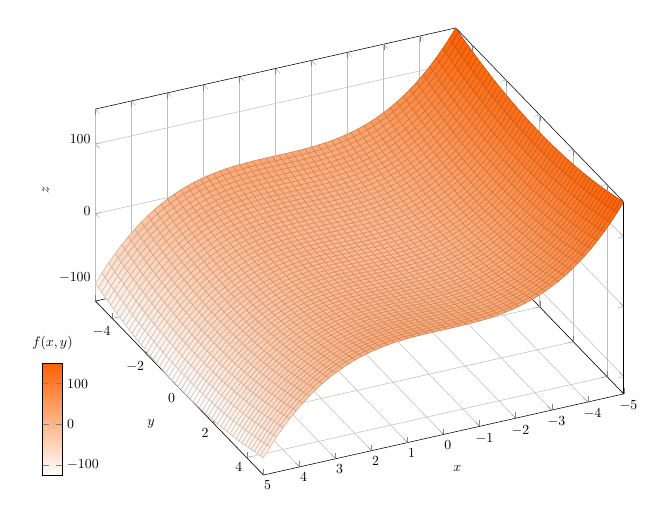
\begin{tikzpicture}[scale=0.5]
    \begin{axis}[
    colormap name=whitered,
    width=15cm,
    view={155}{45},
    enlargelimits=false,
    grid=major,
    domain=-5:5,
    y domain=-5:5,
    samples=56, %57 : TeX capacity exceeded, sorry [main memory size=3000000].
                % see also http://tex.stackexchange.com/a/7954/5645
    xlabel=$x$,
    ylabel=$y$,
    zlabel={$z$},
    colorbar,
    colorbar style={
        at={(-0.1,0)},
        anchor=south west,
        height=0.25*\pgfkeysvalueof{/pgfplots/parent axis height},
        title={$f(x,y)$}
    }
    ]
      \addplot3[surf] {y*y-x*x*x};
    \end{axis} 
\end{tikzpicture}
